Para a criação de um tarefa de aprendizado que seja capaz de verificar a autenticidade de assinaturas de indivíduos, é necessário primeiramente a existência de um conjunto de dados de imagens que possuam exemplos de assinaturas forjadas e genuínas. Para isto, utilizou-se o conjunto de dados da 

\begin{figure}[h!]
\centering
\caption{Uma amostra das assinaturas on-line e off-line. Font: \cite{icdar2009}}
\label{fig:sample-signature}
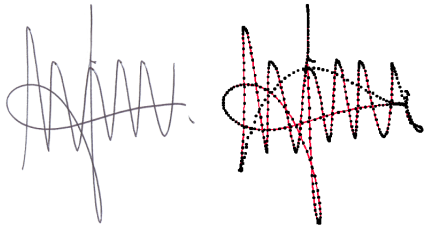
\includegraphics[width=0.6\textwidth]{imgs/sample-signature}
\end{figure}
